\chapter{Software Architektur}
\label{sec:software-architektur}

Die Software-Architektur des Projektes definiert die Möglichkeiten bei der Implementierung, die man zum Erfüllen der Anforderungen zur Verfügung hat. Deshalb war es wichtig, sich ausreichend Gedanken zu machen, um später im Projekt nicht feststellen zu müssen, dass die gewählte Architektur für die Anforderungen ungeeignet ist. Die Hauptanforderung an die Architektur ist selbstverständlich die Bereitstellung eines Kommunikationskanals zwischen Controllern und Robotern. Es muss möglich sein Richtungs- und Geschwindigkeitsänderungen seitens der Anwender rechtzeitig an die Roboter mitzuteilen. Interaktivität spielt hierbei eine große Rolle. Die getätigten Steuerungen sollen möglichst zeitnah umgesetzt werden, damit der Benutzer ein gutes Feedback auf seine Steuerung erhält, auch wenn der Roboter eine hohe Geschwindigkeit hat. Der Status des Roboters soll von der Steuerlogik jederzeit ausgewertet und entsprechend darauf reagiert werden können. Hierzu gehören das automatische Anfahren der Ladestation bei geringem Akkustand und die Übertragung der Bilddaten. Außerdem sollen Zustandsänderungen des Spiels, die nicht vom Roboter oder Controller direkt ausgehen erkannt und korrekt verarbeitet werden. Der Nutzer soll lediglich die Informationen Akkustand, Spielstand und die Kameraübertragung zugeteilt bekommen. Alles weitere ist Aufgabe der Steuerlogik und soll vom Nutzer abstrahiert werden. Dadurch entsteht eine klare Rollenverteilung: Der Roboter nimmt lediglich Befehle für die Motoren und den Schussapparat an und der Steuercontroller bekommt Informationen, um mit dem Nutzer interagieren zu können.

Die betrachteten Architekturen waren folgende:

Eine \textbf{Client-Server-Architektur} bei der ein Server zentral die Kommunikation verwaltet. Hierbei findet keine Kommunikation zwischen den Steuergeräten und den Robotern direkt statt. Die Torerkennung kommuniziert direkt mit dem Server, ohne dass Roboter und Controller zwangsweise etwas davon mitbekommen. Sowohl die Roboter, als auch die Controller nehmen die Rolle eines Clients ein. Dadurch ist es Möglich, dass eine Steuerung des Servers stattfinden kann, ohne dass ein Controller verbunden ist. Der Server verwaltet zentral alle Informationen von Steuercontroller und Roboter und leitet nur diejenigen weiter, die für den anderen relevant sind. Dadurch wird ein Steuercontroller wirklich nur zu einem Gerät, mit dem der Roboter gesteuert werden kann und das sonst keine weitere Logik enthält. Zusätzlich ist es in dieser Architektur möglich beliebig viele Clients anzubinden. Durch die Trennung von Client und Logik können die Controller beliebig erweitert und ausgetauscht werden, ohne die eigentliche Spiellogik zu ändern.


Eine Architektur, die Roboter und Controller \textbf{paarweise} verbindet. Bei dieser Architektur wird jedem Roboter ein Controller zugewiesen, der genau diesen steuert. Die peripheren Geräte senden direkt an die Controller. Auch die gesamte Spiellogik ist in den Controller gekapselt. Ein Vorteil dieser Architektur ist die geringe Latenz bei der Befehlsübermittlung. Im Vergleich zur Client-Server-Architektur gibt es hier keinen dritten Knoten, über den die Übertragung abgehalten wird, wodurch sich die benötigte Zeit halbiert. Dies stellt für die Rechtzeitigkeit der Steuerung einen erheblichen Vorteil dar. In Bezug auf die Rollenverteilung hat diese Architektur jedoch gravierende Nachteile. Wenn die gesamte Steuerlogik in die Steuercontroller integriert ist, kann der Roboter auch nur dann agieren, wenn ein Steuercontroller verbunden ist. Das Anfahren der Ladestation wäre dadurch erst möglich, sobald sich ein Nutzer verbindet.

\vspace{1cm}

\begin{figure}[h!]
	\centering
	\begin{subfigure}{0.45\textwidth}
		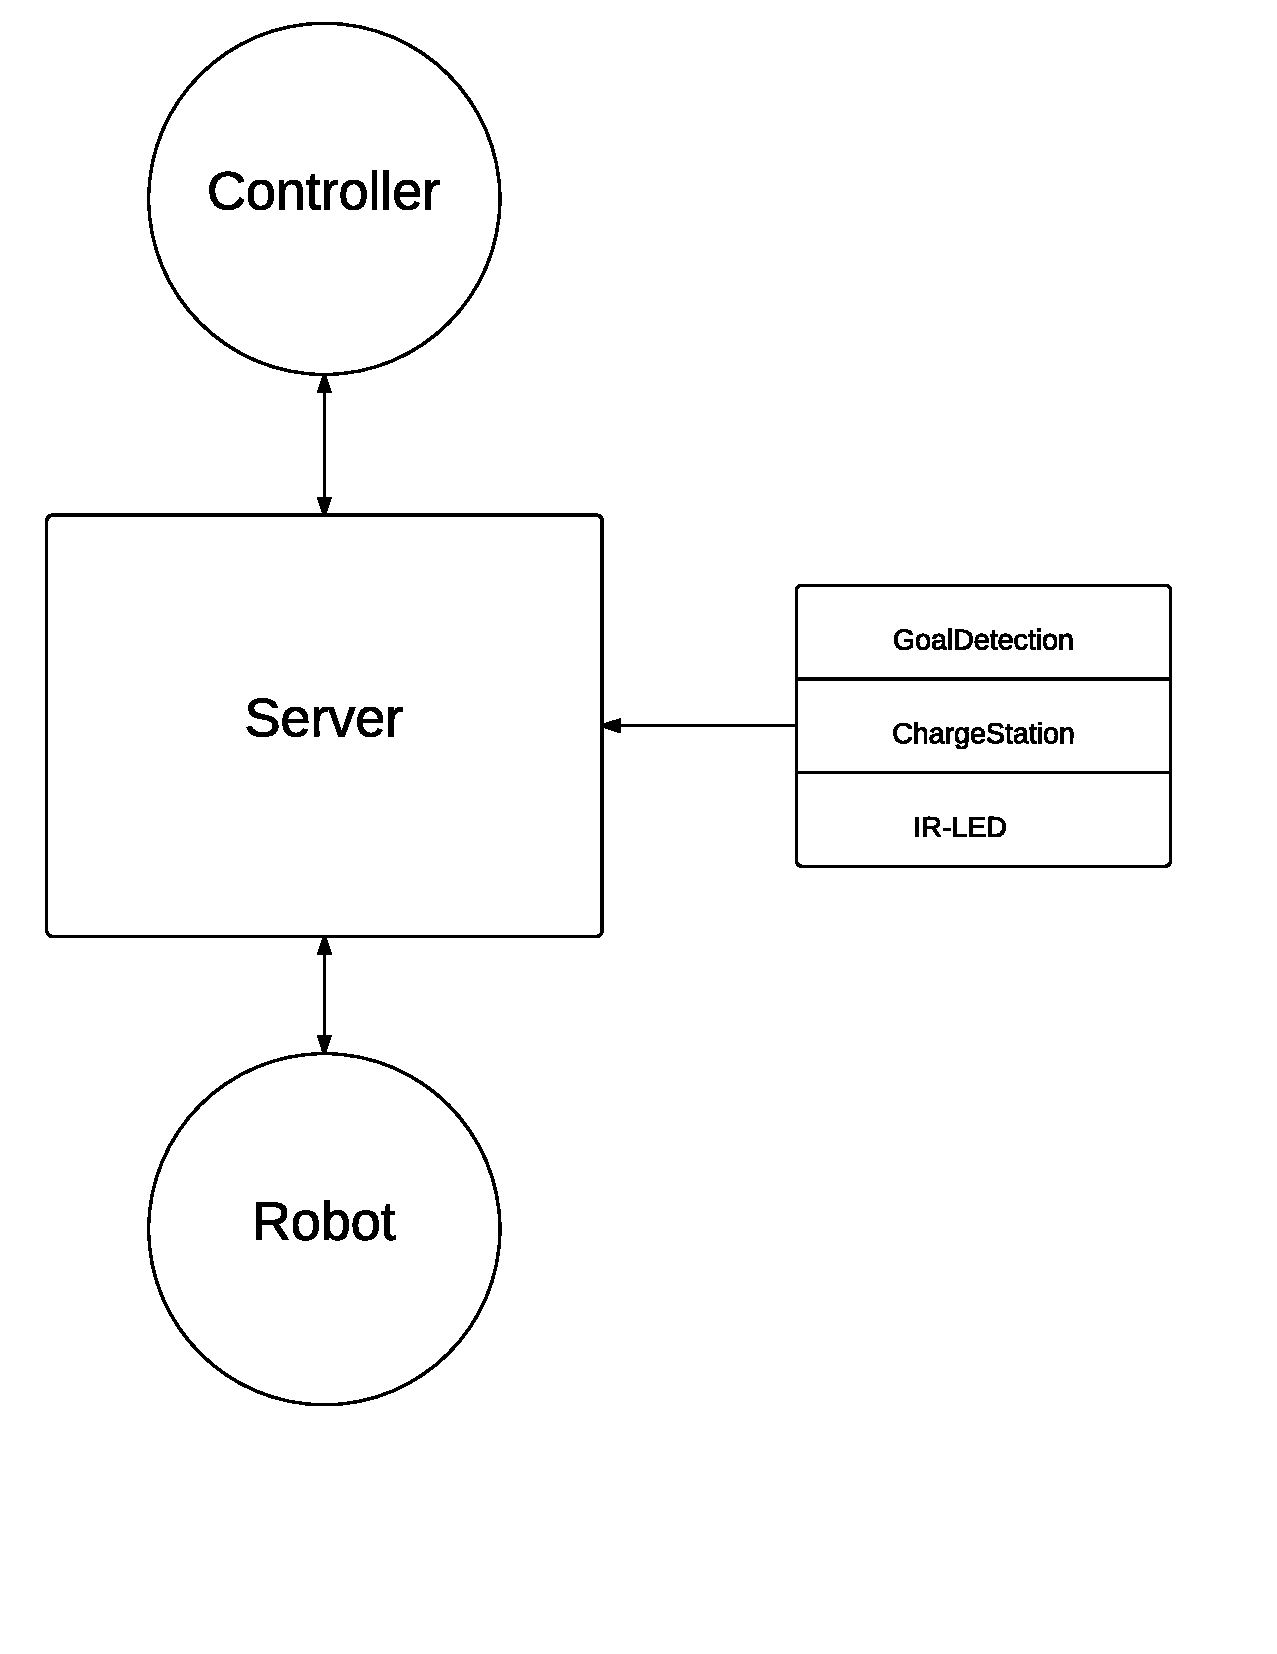
\includegraphics[height = 8cm]{images/client-server_architektur.pdf}
		\caption{Client-Server Architektur}
		\label{fig:client-server_architektur}
	\end{subfigure}
	\quad
	\begin{subfigure}{0.45\textwidth}
		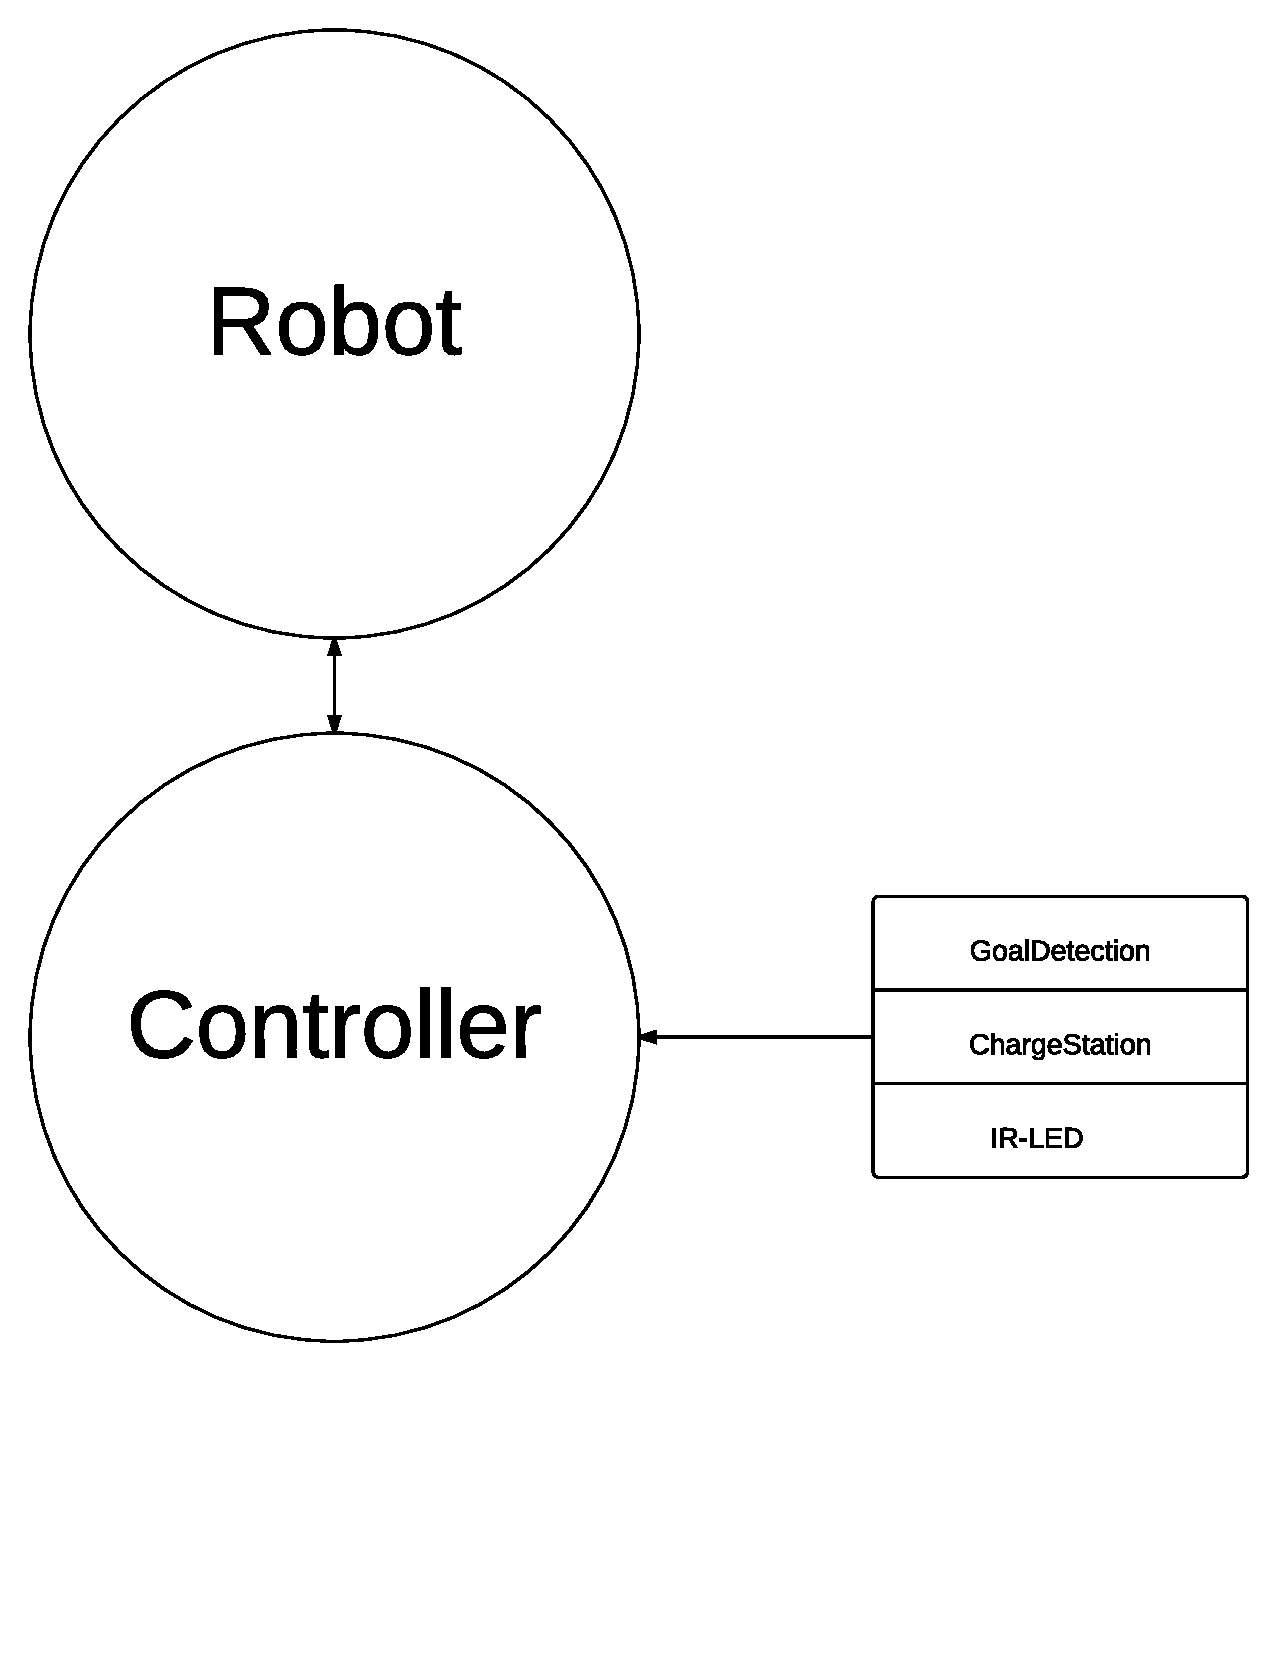
\includegraphics[height = 8cm]{images/paarweise_architektur.pdf}
		\caption{Paarweise Architektur}
		\label{fig:paarweise_architektur}
	\end{subfigure}
	
	\caption{Mögliche Architekturen}
\end{figure}
\vspace{1cm}


Nach Abwägung der Vor- und Nachteile beider Architekturen schien es vernünftiger sich für die Client-Server-Architektur zu entscheiden. Die Hauptgründe hierfür sind die hervorragende Erweiterbarkeit in Bezug auf die Controller und die klare Rollenverteilung. Da keine Logik in den Controllern ist, muss sie auch nicht für jeden Controller separat entwickelt werden, beziehungsweise nicht einmal vorhanden sein. Das spielt unter Betrachtung von Abschnitt \ref{sec:wahl_endgeraete} eine wichtige Rolle um die Webanwendung gut integrieren zu können. Für das Auffinden der Ladestation wäre es nicht sinnvoll, solange mit dem Laden zu warten, bis ein Controller verbunden ist, nur um dann festzustellen dass der Akku leer ist und der Roboter erst geladen werden muss, bevor gespielt werden kann. Auch in Anbetracht der Informationskapselung, die bei der paarweisen Architektur entstehen würde, ist es sinnvoller die Client-Server-Architektur zu bevorzugen. In Anbetracht der Rechtzeitigen Steuerung bietet die gewählte Architektur einen Nachteil gegenüber der paarweisen, da eine dritte Komponente in der Übertragungskette vorhanden ist und deshalb doppelt so viele Pakete versendet werden müssen. Jedoch wird sich später bei der Implementierung herausstellen, dass die Übertragungsgewschwindigkeit auch bei der Client-Server Architektur hoch genug ist, um eine für den Benutzer verzögerungsfreie Steuerung zu gewährleisten.